
%%% Local Variables: 
%%% mode: latex
%%% TeX-master: t
%%% End: 

\chapter{基于 $k$-CBP 碰撞检测算法}
\label{cha:kcbp-collision-detection}

碰撞检测算法是计算机图形学、计算机动画等领域里必不可少的。
本章提出了基于~$k$-CBP~的碰撞检测算法,算法首先对输入的网格模型进行预处理,构造模型的~AABB~包围体、$k$-CBP,
当进行碰撞检测时,首先判断~AABB~是否相交,若相交再进行~$k$-CBP~之间的相交测试,再次相交再进行实际模型的相交测试。再进行实际模型的相交测试时,利用了~AABB~树形结构进行判断剪枝。
在凸包围~$k$~面体之间分别用~AABB~树的方式和基于~GJK~算法两种方式进行,实验结果表明本文提出的方法能够有效加速碰撞检测算法。

本章后续部分的内容组织如下:
第一小节介绍~$k$-CBP~之间的相交测试算法,
第二小节介绍三角网格的相交测试算法,
第三节介绍总体的算法流程,
最后一节为实验结果的分析。


\section{$k$-CBP 的相交测试算法}
\label{sec:kcbp:cd}

在所有基于包围体的碰撞检测算法中,都是利用了包围体的相交测试比直接用原始模型相交测试更简单以提升算法的整体效率,包围体的相交测试是非常重要的一个步骤。
与其他基于包围体的碰撞检测算法一样,本文基于~$k$-CBP~的算法也是先进行~$k$-CBP~的相交测试,若~$k$-CBP~相交,再进行原始模型的相交测试。
$k$-CBP~之间的相交测试以两种方法实现,一种是将构造的~$k$-CBP~进行空间划分,构造~$k$-CBP~的~AABB~树,再基于~AABB~树进行相交测试,详细划分原则等算法见第~\ref{subsec:kcbp:cd:aabb}~;
另一种是基于凸多面体的相交测试算法~GJK~,详细算法见第~\ref{subsec:kcbp:cd:gjk}节。

\subsection{基于 AABB 树的算法}
\label{subsec:kcbp:cd:aabb}

AABB~包围体是碰撞检测算法过程中一种常用的包围体,构造模型的~AABB~包围体树能够有效提高模型的求交或碰撞检测过程。
本文将构造得到的~$k$-CBP~视为普通的三角网格模型,采取一种自上而下的构造~AABB~包围体树的方法,顶层包围体为所有三角网格的包围体的并集,然后按照包围体跨度最大的维度进行划分成两个子节点,然后再对每个子节点进行递归划分。
具体算法如算法~\ref{alg:aabbtree:build}~所示。

\begin{algorithm}[htbp]
\small
\caption{AABB~树的构造}
\label{alg:aabbtree:build}
\begin{algorithmic}[1]
\Require
原始三角网格 $primitives$ 和下标 $first, last$
\Ensure
AABB~树的根节点 $root$

\Function{ConstructAABBTree}{$primitives, first, last$}
  \State $root \gets \Call{constructNode()}{}$ 
  \State $root.primitives \gets primitives$
  %\State $root.box \gets \emptyset $
  \For{$i = first \to last$}
      \State $root.box \gets root.box \cup primitives[i].box$
      \Comment{求每个三角网格的~AABB~的并集}
  \EndFor

  \State $size \gets primitives.size$  
  \If {$size = 1$}
  \State \Return $root$
  \EndIf

  \State $axis \gets \Call{longestAixs}{root.box}$
  \Comment {计算包围体跨度最大的轴}
  \State {$\Call{sort}{primitives, axis}$}
  \Comment {按照 $axis$ 对 $primitives$ 排序}
  
  \If {$size = 2 $}
      \State  {$root.left \gets \Call{constructNode()}{}$}
      \State  {$root.left.primitives \gets primitives[0]$}
      \State  {$root.left.box \gets primitives[0].box$}
      \State  {$root.right \gets \Call{constructNode()}{}$}
      \State  {$root.right.primitives \gets primitives[1]$}
      \State  {$root.right.box \gets primitives[1].box$}
      \State \Return $root$
  \EndIf
  \State $half \gets size / 2 $
  \State $root.left \gets \Call{ConstructAABBTree}{primitives, first, half}$
  \State \Comment{前一半作为其中一个叶子节点,继续递归构造}
  \State $root.right \gets \Call{ConstructAABBTree}{primitives, half+1, size}$ \Comment{后一半继续递归构造}
  \State \Return $root$
\EndFunction
\end{algorithmic}
\end{algorithm}

为了使生成的~AABB~包围体树更加平衡,因此划分策略为两个子节点包含相同数量的三角网格。划分轴采用沿着坐标轴方向节点跨度最大的轴进行划分,在对三角网格进行排序时,通常可选择三角网格中心位置的某轴向坐标值进行排序,
因为本文的策略为平衡二叉树策略,两个孩子节点包含三角网格数量一致,因此该点的选择不会对总体划分产生较大影响,只会影响划分轴边缘的三角网格,因此本文仅仅简单选择三角网格第一个坐标点的轴向坐标轴进行排序。

假设算法~\ref{alg:aabbtree:build}~的时间复杂度为~$T(n)$~,则有
\begin{equation}
  T(n) = O(n \log n ) + 2T(\frac{n}{2}),
\label{equa:aabbtree:build}
\end{equation}
公式~\ref{equa:aabbtree:build}~中~$O(n \log n)$~为算法中根据某坐标轴排序的耗费,根据主定理得此构造包围体树的整体算法时间复杂度~$T(n)=O(n\log^2n)$~,文献~\onlinecite{ericson2005real}~中提到可以用一种~$O(n)$~的算法替代其中的排序操作,使得整体复杂度为~$O(n\log n)$。

生成两个~$k$-CBP~的~AABB~包围体树后,当进行碰撞检测时,将采用如下的迭代算法进行判断。从顶层~AABB~节点开始,若两个节点的~AABB~包围体相交,则进行深度优先遍历其孩纸节点,当到达叶子节点时,再进行原生几何(本文中的~$k$-CBP~多边形网格,为了方便转化成与输入模型一致的三角网格)进行相交测试的判断,$k$-CBP~相交后,进行真实模型的相交测试也通过此方法进行。

\begin{algorithm}[htbp]
\small
\caption{基于AABB~树碰撞检测迭代算法}
\label{alg:aabbtree:traverse:iterator}
\begin{algorithmic}[1]
\Require
两棵~AABB~树的根节点 $rootA, rootB$
\Ensure
是否相交

\Function{TraverseDetective}{$rootA, rootB$}
  \State $p \gets \Call{initStack}{}, q \gets \Call{initStack}{}$  \Comment{初始化两个栈,用于记录待判断的~AABB~节点对}
  \State $p.\Call{Push}{rootA}, q.\Call{Push}{rootB}$  
  
  \While {$! p.\Call{empty()}{} ~~\textbf{and}~~ !q.\Call{empty()}{}$}
      \State $nodeA \gets p.\Call{Pop()}{}$
      \State $nodeB \gets q.\Call{Pop()}{}$
      \State $c \gets \Call{Intersect}{nodeA.box, nodeB.box}$ \Comment {判断两个节点的~AABB~包围体是否相交}
      \If {$c = \textbf{False}$}
          \State \textbf{Continue} /Comment{节点~AABB~不相交,则过滤到这两个节点及其孩子节点}
      \EndIf
      \If {$nodeA.\Call{isLeaf()}{}$}
          \If {$nodeB.\Call{isLeaf()}{}$}
              \Comment{两个叶子节点的原始几何进行相交测试} 
              \ForAll {$p_1 \in nodeA.primitives$}
                  \ForAll {$p_2 \in nodeB.primitives$}
                      \If {$\Call{Intersect}{p_1, p_2} = \textbf{True} $}
                          \State \Comment {按照第~\ref{sec:intersection:triangles}~节中的算法进行原始三角网格相交测试}
                          \State \Return \textbf{True} \Comment{若相交就直接返回True}
                      \EndIf
                  \EndFor
              \EndFor
          \Else  \Comment{nodeB~节点有孩子节点}
              \State $p.\Call{push}{nodeA}, q.\Call{push}{nodeB.left}$
              \State $p.\Call{push}{nodeA}, q.\Call{push}{nodeB.right}$
          \EndIf
      \Else \Comment{nodeA~节点有孩子节点}
          \If {$nodeB.\Call{isLeaf()}{}$}
              \Comment{nodeB~是叶子节点}
              \State $p.\Call{push}{nodeA.left}, q.\Call{push}{nodeB}$
              \State $p.\Call{push}{nodeA.right}, q.\Call{push}{nodeB}$
          \Else
              \Comment{nodeA~和~nodeB~都有叶子节点} 
              \State $p.\Call{push}{nodeA.left}, q.\Call{push}{nodeB.left}$
              \State $p.\Call{push}{nodeA.left}, q.\Call{push}{nodeB.right}$
              \State $p.\Call{push}{nodeA.right}, q.\Call{push}{nodeB.left}$
              \State $p.\Call{push}{nodeA.right}, q.\Call{push}{nodeB.right}$
          \EndIf
      \EndIf
  \EndWhile
  \State \Return \textbf{False} \Comment{遍历完毕也没有检测到原始三角网格相交,则返回False}
\EndFunction
\end{algorithmic}
\end{algorithm}

算法~\ref{alg:aabbtree:traverse:iterator}~中,底层叶子节点包含的原始三角网格数量与树的高度相关,对于相同的模型,树的高度越低,叶子节点包含三角网格数量也就越多,
且叶子节点测试的时间复杂度为~$O(m^2)$,$m$~为叶子节点包含的三角网格数量,一般而言在存储允许的情况下都尽量使得最底层叶子节点仅包含1个或少数几个三角形,以减少底层叶子节点三角网格两两测试的时间复杂度。

当在运动场景中的模型进行碰撞检测时,需要对~$k$-CBP及模型的~AABB~包围体树进行更新,本文采用一种近似的算法进行计算,详细将在第~\ref{sec:cd:baseon:kcbp}~节中介绍。

\subsection{基于 GJK 的算法}
\label{subsec:kcbp:cd:gjk}



\section{三角网格的相交测试算法}
\label{sec:intersection:triangles}




\section{基于 $k$-CBP 的碰撞检测算法}
\label{sec:cd:baseon:kcbp}

凸包围多面体可应用于加速相关几何算法的整体效率, 图~\ref{lbl:bunny-box-kcbp-collsion-detection-example}
为利用~Bunny~模型进行碰撞检测的示例, 图中模型~1~与~2、2~与~3~的包围盒分别相交, 而其~$16$-CBP~仅~1~与~2~相交, 实际模型仅~1~与~2~相交.
用~$16$-CBP~可排除模型~2~与~3~之间的碰撞检测, 而仅用包围盒算法则无法排除, 显然检测模型~2~与~3~的~$16$-CBP~是否相交比直接通过检测模型~2~与~3~是否相交更省时间.
%在碰撞检测算法中, 在进行真实模型的相交检测前一般会用包围球、包围盒等包围体进行预先排除$^{[17]}$.

\begin{figure}[htbp] 
\centering
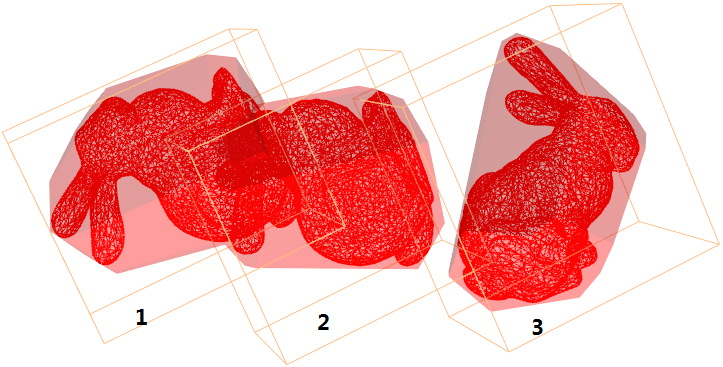
\includegraphics[width=4.5in]{bunny-box-kcbp-collsion-detection-example.png}
\caption{~$k-$CBP~应用于碰撞检测示例}
\label{lbl:bunny-box-kcbp-collsion-detection-example}
\end{figure}


模型的~$k$-CBP~相交后,会用模型的~AABB~树进一步对模型进行碰撞检测,模型的~AABB~树构造方法如第~\ref{subsec:kcbp:cd:aabb}~节所述,
图~\ref{fig:bunny:aabb:bvh:toplayer4}~是按照本文所采用的构造方法针对~Bunny~模型构造的~AABB~树形结构的顶上~4~层。

\begin{figure}[htpb]
  \centering
  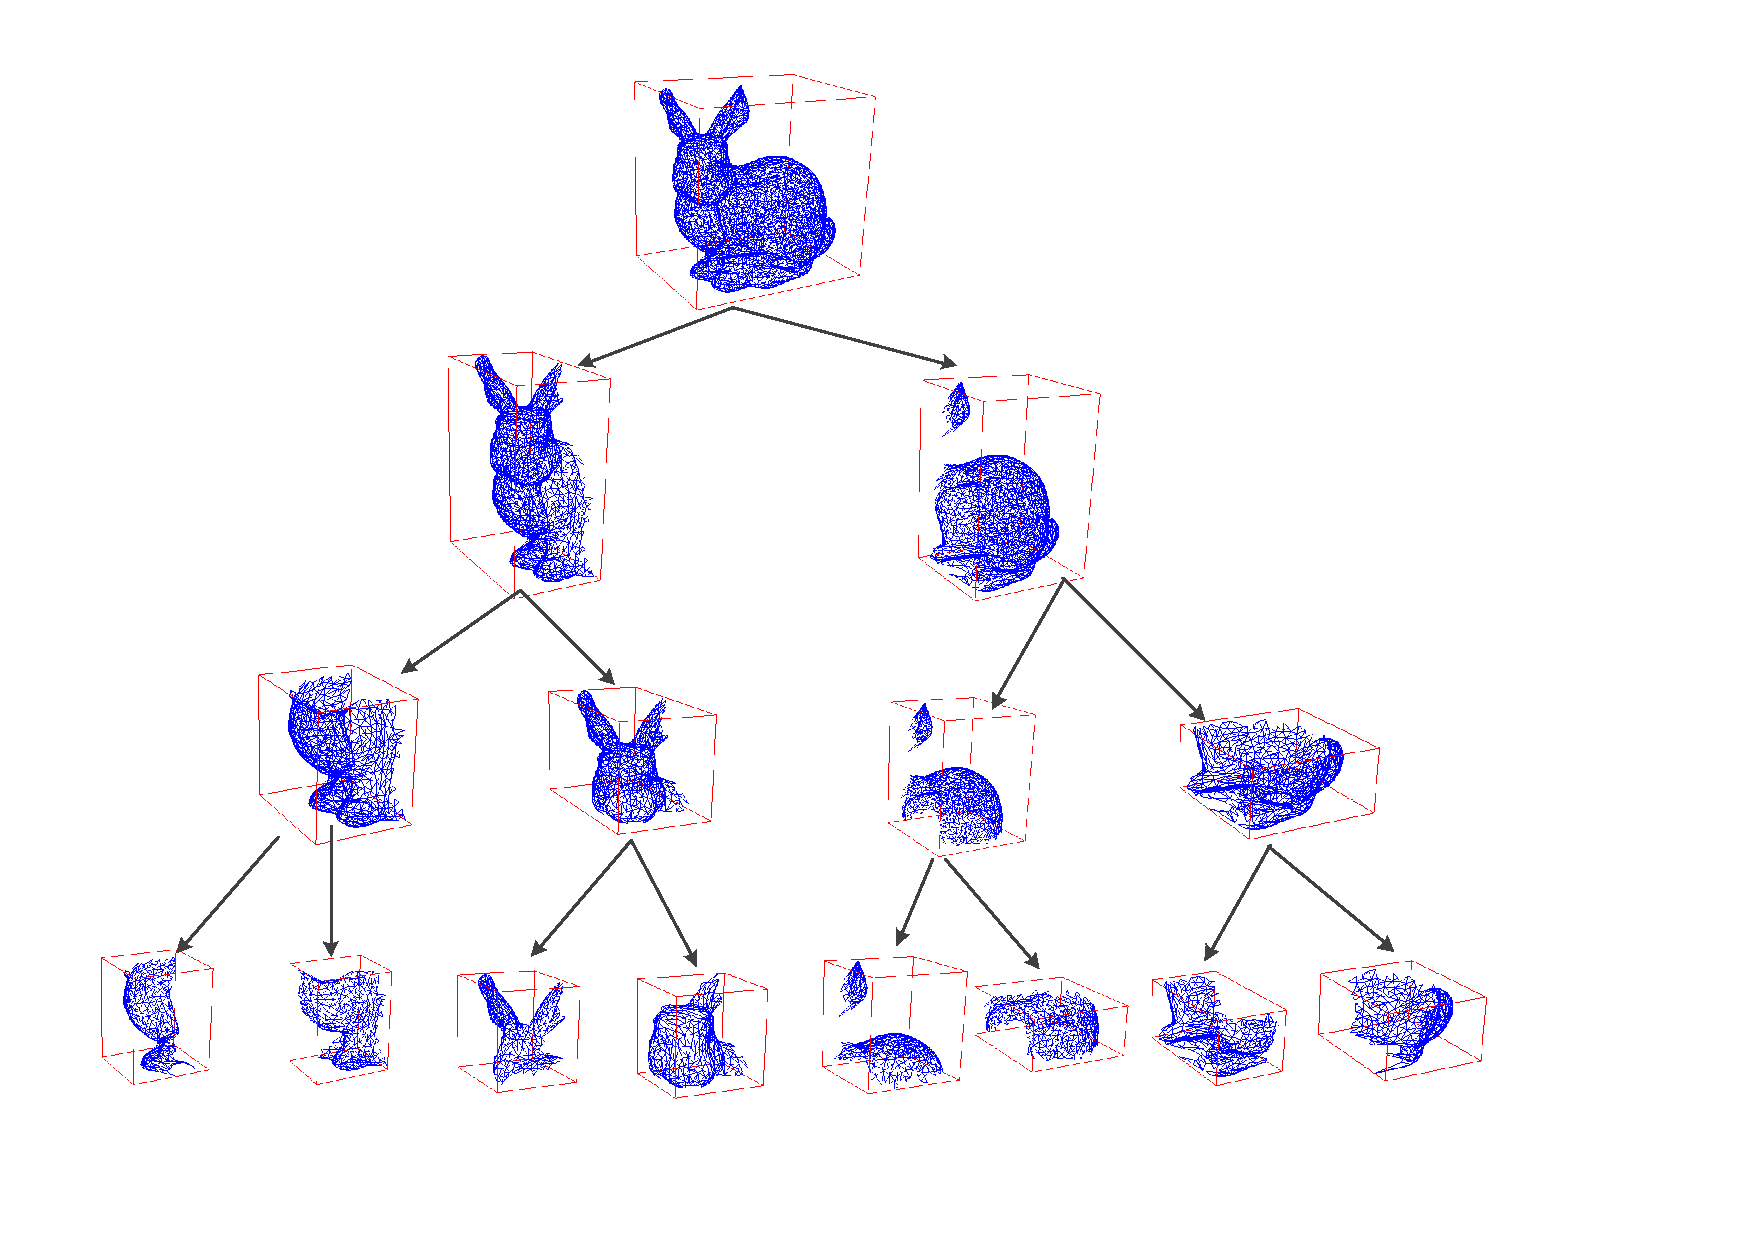
\includegraphics[width=\textwidth]{bunny-aabb-bvh-4-layers.pdf}
  \caption{Bunny~模型的~AABB~树形结构(部分)}
  \label{fig:bunny:aabb:bvh:toplayer4}
\end{figure}



动态场景

当运动场景中的模型进行碰撞检测时,需要更新

模型围绕任意轴~$\bm{n}(x, y, z)$~旋转任意角度~$\theta$~的变换矩阵如公式~\ref{equa:rotate:matrix}~所示,其中$\phi = 1-\cos\theta$
详细的推导过程可以参考文献~\onlinecite{dunn20023d}。

\begin{equation}

  
\bm{R}(\bm{n},\theta)= \\\\
%\left\{
\begin{pmatrix}
  %\begin{array}{ccc}
    %\cos\theta+(1-\cos\theta)\cdot\bm{n}_x^2 & (1-\cos\theta)\cdot\bm{n}_x\cdot\bm{n}_y + \sin\theta\cdot\bm{n}_z & (1-\cos\theta)\cdot\bm{n}_x\cdot\bm{n}_z-\sin\theta\cdot\bm{n}_y \\
    %(1-\cos\theta)\cdot\bm{n}_x\cdot\bm{n}_y-\sin\theta\cdot\bm{n}_z & \cos\theta+(1-\cos\theta)\cdot\bm{n}_y^2 & (1-\cos\theta)\cdot\bm{n}_y\cdot\bm{n}_z+\sin\theta\cdot\bm{n}_x \\
    %(1-\cos\theta)\cdot\bm{n}_x\cdot\bm{n}_z + \sin\theta\cdot\bm{n}_y & (1-\cos\theta)\cdot\bm{n}_y\cdot\bm{n}_z - \sin\theta\cdot\bm{n}_x &  \cos\theta+(1-\cos\theta)\cdot\bm{n}_z^2 
    \cos\theta+\bm{n}_x^2\phi & \bm{n}_x\bm{n}_y\phi + \bm{n}_z\sin\theta & \bm{n}_x\bm{n}_z\phi-\bm{n}_y\sin\theta \\
    \bm{n}_x\bm{n}_y\phi - \bm{n}_z\sin\theta & \cos\theta+\phi\bm{n}_y^2 & \bm{n}_y\bm{n}_z\phi+\bm{n}_x\sin\theta \\
    \bm{n}_x\bm{n}_z\phi + \bm{n}_y\sin\theta & \bm{n}_y\bm{n}_z\phi - \bm{n}_x\sin\theta &  \cos\theta+\bm{n}_z^2\phi 
  %\end{array}
%\right\}
\end{pmatrix}

\label{equa:rotate:matrix}
\end{equation}

\section{实验结果}
\label{sec:exper-cd}

[TODO]


本文实验通过生成不同数量的模型(模型位置和旋转角度随机生成), 碰撞检测时首先判断包围盒是否相交, 然后判断凸包围多面体是否相交, 最后再判断实际模型是否相交.
凸包围多面体之间的碰撞检测时可采用文献~${[27]}$~中提到的方法,
本文案例中模型和凸包围多面体是否相交都采用了普通~AABB~树的方式进行判断,
从如表~\ref{tab:exp:box:kcbp:collsiondetection}~的实验结果可看出含有凸包多围体的模型之间的碰撞检测算法能显著提高整体应用的效率. 

%\begin{landscape} 横放,效果不好看, 还是将表头的单位去掉了
\begin{table}[htbp]
\caption{$k$-CBP~和包围盒应用于碰撞检测结果对比}
\label{tab:exp:box:kcbp:collsiondetection}
\centering
\begin{tabular}{lccccccl}
 \toprule[1.5pt]
  n& c(Box) & c($16$-CBP) &  t(Box) & t($16$-CBP) & r(Box) & r($k$-CBP) & n(Model) \\
  \midrule[1.0pt]
%  10 & 0.1 & 1.8 & 26.0  & 0.1 & 2 & 0 & 0\\
%  30 & 0.2 & 2.9 & 134.0  & 70.0 & 11 & 6 & 5\\
%  50 & 0.5 & 4.8 & 506.0  & 255.2 & 41 & 22 & 19 \\
%  70 & 0.4 & 4.8 & 901.1  & 492.5 & 77 & 42 & 34 \\
%  90 & 0.7 & 5.7 & 1324.0  & 734.7 & 110 & 63 & 46 \\
%  100 & 0.7 & 7.8 & 1481.0  & 870.7 & 127 & 73 & 55 \\
%  150 & 1.0 & 9.8 & 4153.1  & 2473.0 & 349 & 212 & 150 \\
%  200 & 1.6 & 12.8 & 8049.3 & 4430.9 & 685 & 394 & 281 \\
   10 & 0.1 & 1.8 &    26.0  & 0.1    & 0.00  & 100.00 & 0\\
   30 & 0.2 & 2.9 &   134.0  & 70.0   & 45.45 & 83.33 & 5\\
   50 & 0.5 & 4.8 &   506.0  & 255.2  & 46.34 & 86.36 & 19 \\
   70 & 0.4 & 4.8 &   901.1  & 492.5  & 44.16 & 80.95 & 34 \\
   90 & 0.7 & 5.7 &  1324.0  & 734.7  & 41.82 & 73.02 & 46 \\
  100 & 0.7 & 7.8 &  1481.0  & 870.7  & 43.31 & 75.34 & 55 \\
  150 & 1.0 & 9.8 &  4153.1  & 2473.0 & 42.98 & 70.75 & 150 \\
  200 & 1.6 & 12.8 & 8049.3  & 4430.9 & 41.02 & 71.32 & 281 \\
  \bottomrule[1.5pt]
 \end{tabular}
\end{table}
%\end{landscape}


[TODO]构造kcbp的时间 是得到一个后直接rotate顶点得到新的 总时间。且project是GPU的时间。

如表~\ref{tab:exp:box:kcbp:collsiondetection}~所示,
其中~n~表示场景中模型的数量, c(Box), c($16$-CBP)分别表示模型包围盒的构造时间和凸包围16面体的构造时间(单位ms), t(Box), t($16$-CBP)~分表表示用包围盒进行碰撞检测和利用凸包围16面体进行碰撞检测所耗费的时间,
其中~r(Box), r($16$-CBP)分别表示包围盒、16-CBP~的命中率(即用实际模型相交的数量除以包围体检测出来相交的数量), ~n(Model)模型实际相交的数量, 显然计算模型包围盒所耗费的时间要明显少于计算凸包围多面体的时间, 但由于凸包围多面体比包围盒紧致,
因而命中率比包围盒高, 能排除更多本不相交的模型进而节省碰撞检测总时间, 提高算法效率.


为了和K-DOP进行对比,相同模型,kcbp也与kdop一样扫描点击重新构造,且都是用CPU实现的算法。
